\documentclass[tikz,border=2mm]{standalone}
\usepackage{tikz}
\usepackage{xcolor}
\usepackage{graphicx}
\usepackage{url}
\usepackage{color}
\usepackage{varwidth}
\usepackage{Sweave}
\tikzset{font={\fontsize{12pt}{12}\selectfont}}
\usepackage{helvet}
\IfFileExists{sfmath.sty}{\RequirePackage[helvet]{sfmath}}{}
\renewcommand{\sfdefault}{phv}
\renewcommand{\rmdefault}{phv}
\begin{document}
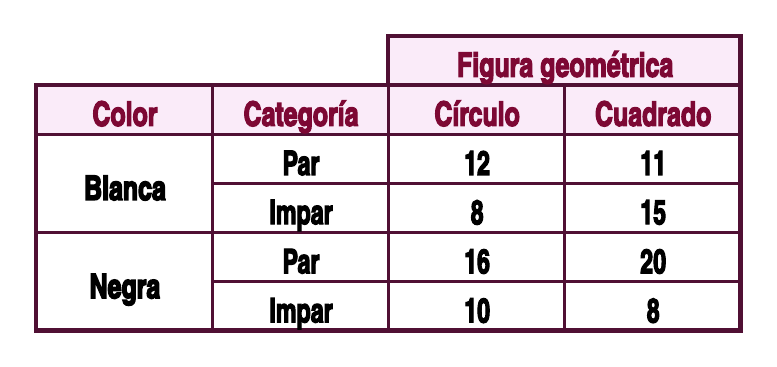
\begin{tikzpicture}[x=0.5pt,y=-0.5pt]
\makeatletter
\definecolor{tfRelleno}{RGB}{250,235,249}
\definecolor{tfVino}{RGB}{125,8,52}
\definecolor{tfLinea}{RGB}{80,16,52}
\def\tfFB{\fontsize{12.2pt}{12.2pt}\fontseries{bc}\pgfutil@selectfont}
\def\tfsxH{0.90}\def\tfsxK{0.90}\def\tfsxR{0.84}
\def\tfeH{0.45}\def\tfeK{0.55}\def\tfeR{0.45}
\def\tfEon#1{\pgfsys@invoke{2 Tr #1 w}}
\def\tfEoff{\pgfsys@invoke{0 Tr}}
\def\tfTgen#1#2#3#4#5#6#7{\begin{scope}[shift={(#1,#2)},xscale=#3,transform shape]\node[anchor=base,inner sep=0pt,outer sep=0pt,font=#4,text=#5] at (0,0) {#6#7\tfEoff};\end{scope}}
\def\tfTH#1#2#3{\tfTgen{#1}{#2}{\tfsxH}{\tfFB}{tfVino}{\tfEon{\tfeH}}{#3}}
\def\tfTK#1#2#3{\tfTgen{#1}{#2}{\tfsxK}{\tfFB}{black}{\tfEon{\tfeK}}{#3}}
\def\tfTR#1#2#3{\tfTgen{#1}{#2}{\tfsxR}{\tfFB}{black}{\tfEon{\tfeR}}{#3}}
\ifdefined\tfmw\else\newlength{\tfmw}\fi
\def\tfpad{9}\def\tfNecC{0}\def\tfNecT{0}
\def\tfMedC#1#2#3{\settowidth{\tfmw}{#1 #3}\pgfmathsetmacro\tfNecC{max(\tfNecC,2*\tfmw*#2+2*\tfpad)}}
\def\tfMedT#1#2#3{\settowidth{\tfmw}{#1 #3}\pgfmathsetmacro\tfNecT{max(\tfNecT,2*\tfmw*#2+2*\tfpad)}}

\tfMedT{\tfFB}{\tfsxH}{Figura geométrica}
\tfMedC{\tfFB}{\tfsxH}{Color}
\tfMedC{\tfFB}{\tfsxK}{Blanca}
\tfMedC{\tfFB}{\tfsxR}{Par}
\tfMedC{\tfFB}{\tfsxR}{Impar}
\tfMedC{\tfFB}{\tfsxR}{12}
\tfMedC{\tfFB}{\tfsxR}{8}
\tfMedC{\tfFB}{\tfsxR}{16}
\tfMedC{\tfFB}{\tfsxR}{10}
\tfMedC{\tfFB}{\tfsxR}{11}
\tfMedC{\tfFB}{\tfsxR}{15}
\tfMedC{\tfFB}{\tfsxR}{20}
\tfMedC{\tfFB}{\tfsxR}{8}
\pgfmathsetmacro{\tfW}{max(127.25,\tfNecC,\tfNecT/2)}
\pgfmathsetmacro{\tfxa}{10}\pgfmathsetmacro{\tfxb}{\tfxa+\tfW}\pgfmathsetmacro{\tfxc}{\tfxa+2*\tfW}
\pgfmathsetmacro{\tfxd}{\tfxa+3*\tfW}\pgfmathsetmacro{\tfxe}{\tfxa+4*\tfW}
\pgfmathsetmacro{\tfca}{(\tfxa+\tfxb)/2+0.7}\pgfmathsetmacro{\tfcb}{(\tfxb+\tfxc)/2+0.7}
\pgfmathsetmacro{\tfcc}{(\tfxc+\tfxd)/2+0.7}\pgfmathsetmacro{\tfcd}{(\tfxd+\tfxe)/2+0.7}
\pgfmathsetmacro{\tfct}{\tfxd+0.7}
\fill[white] (\tfxa-6,10) rectangle (\tfxe+6,235);
\fill[tfRelleno] (\tfxc,16) rectangle (\tfxe,51.5);
\fill[tfRelleno] (\tfxa,51.5) rectangle (\tfxe,87);
\begin{scope}[tfLinea,line width=1.05pt,line cap=butt]
\draw (\tfxa,87) -- (\tfxe,87);
\draw (\tfxb,122.5) -- (\tfxe,122.5);
\draw (\tfxa,158) -- (\tfxe,158);
\draw (\tfxb,193.5) -- (\tfxe,193.5);
\draw (\tfxb,51.5) -- (\tfxb,229);
\draw (\tfxc,51.5) -- (\tfxc,229);
\draw (\tfxd,51.5) -- (\tfxd,229);
\end{scope}
\begin{scope}[tfLinea,line width=1.7pt,line join=miter,line cap=butt]
\draw (\tfxc,16) -- (\tfxe,16) -- (\tfxe,229) -- (\tfxa,229) -- (\tfxa,51.5) -- (\tfxc,51.5) -- cycle;
\draw (\tfxc,51.5) -- (\tfxe,51.5);
\end{scope}

\tfTH{\tfct}{45.45}{Figura geométrica}
\tfTH{\tfca}{80.95}{Color}
\tfTH{\tfcb}{80.95}{Categoría}
\tfTH{\tfcc}{80.95}{Círculo}
\tfTH{\tfcd}{80.95}{Cuadrado}
\tfTK{\tfca}{134.50}{Blanca}
\tfTK{\tfca}{205.50}{Negra}
\tfTR{\tfcb}{116.45}{Par}
\tfTR{\tfcc}{116.45}{12}
\tfTR{\tfcd}{116.45}{11}
\tfTR{\tfcb}{151.95}{Impar}
\tfTR{\tfcc}{151.95}{8}
\tfTR{\tfcd}{151.95}{15}
\tfTR{\tfcb}{187.45}{Par}
\tfTR{\tfcc}{187.45}{16}
\tfTR{\tfcd}{187.45}{20}
\tfTR{\tfcb}{222.95}{Impar}
\tfTR{\tfcc}{222.95}{10}
\tfTR{\tfcd}{222.95}{8}
\makeatother
\end{tikzpicture}
\end{document}
